\testfile{pgfplotstest.legend.tex}
\testsection{Legends}
\begingroup
\testsubsection{Old-format legends with two backslashes as separator}
\begin{tikzpicture}
\begin{loglogaxis}[title=A test title,xlabel=Dof,ylabel=Error]
\manylogplotsnolegend
\legend{one\\two\\three\\four\\five\\six\\}%
\end{loglogaxis}
\end{tikzpicture}

\testsubsection{Using comma-separated-legends}
\begin{tikzpicture}
\begin{loglogaxis}[title=A test title,xlabel=Dof,ylabel=Error]
\manylogplotsnolegend
\legend{one,two,three,four,five,six}%
\end{loglogaxis}
\end{tikzpicture}

\testsubsection{testing legend columns}
\begin{tikzpicture}
\begin{loglogaxis}[title=A test title,xlabel=Dof,ylabel=Error,legend columns=2]
\manylogplots
\end{loglogaxis}
\end{tikzpicture}

\begin{tikzpicture}
\begin{loglogaxis}[title=A test title,xlabel=Dof,ylabel=Error,legend columns=3]
\manylogplots
\end{loglogaxis}
\end{tikzpicture}

{
\pgfplotsset{every axis legend/.append style={inner sep=0pt,nodes={inner sep=0pt}}}
\begin{tikzpicture}
\begin{loglogaxis}[title=A test title,xlabel=Dof,ylabel=Error,legend columns=4]
\manylogplots
\end{loglogaxis}
\end{tikzpicture}
}

{\pgfplotsset{every axis legend/.append style={at={(0.5,-0.2)},anchor=north}}
\begin{tikzpicture}
\begin{loglogaxis}[title=A test title,xlabel=Dof,ylabel=Error,legend columns=6]
\manylogplots
\end{loglogaxis}
\end{tikzpicture}
}%

{\pgfplotsset{every axis legend/.append style={at={(0.5,0.98)},anchor=north,inner sep=0pt}}
\begin{tikzpicture}
\begin{loglogaxis}[title=A test title,xlabel=Dof,ylabel=Error,legend columns=-1]
\manylogplots
\end{loglogaxis}
\end{tikzpicture}
}%

\testsubsection{``legend plot pos'' options}
\begin{tikzpicture}
\begin{loglogaxis}[title=A test title,xlabel=Dof,ylabel=Error,legend plot pos=left]
\manylogplots
\end{loglogaxis}
\end{tikzpicture}

\begin{tikzpicture}
\begin{loglogaxis}[title=A test title,xlabel=Dof,ylabel=Error,legend plot pos=right]
\manylogplots
\end{loglogaxis}
\end{tikzpicture}

\begin{tikzpicture}
\begin{loglogaxis}[title=A test title,xlabel=Dof,ylabel=Error,legend plot pos=none]
\manylogplots
\end{loglogaxis}
\end{tikzpicture}


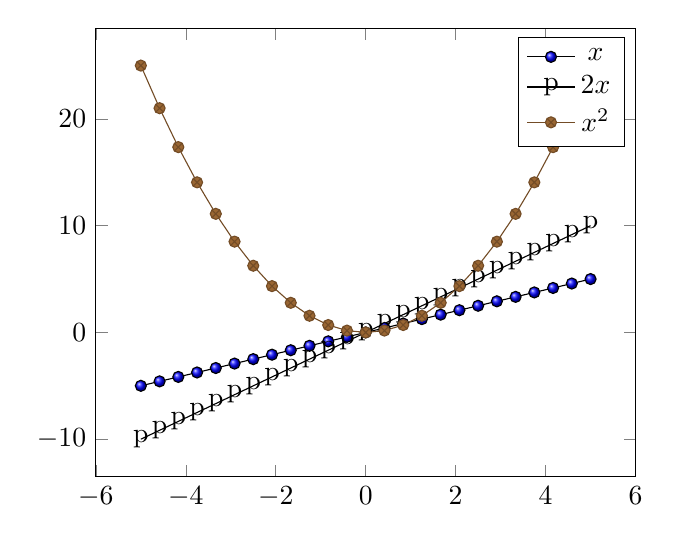
\begin{tikzpicture}
    \begin{axis}[legend entries={$x$,$2x$,$x^2$},]
    \addplot[mark=ball] {x};
    \addplot[mark=text] {2*x};
    \addplot {x^2};
    \end{axis}
\end{tikzpicture}

\endgroup


